\section{Evaluation}
\label{section:evaluation}

%
% power consumption of the ATTiny85
%
\begin{table*}%[h!]
  \begin{center}
  
  \begin{tabular}{| c | c | c |}

  \hline
  \textbf{Mode} & \textbf{Minimum Consumption} & \textbf{Max Consumption} \\
  \hline
  Active      & 0.8 mA & 1.0 mA \\
  Idle        & 0.5 mA & 0.8 mA \\
  Power-Down  & 2 $\mu$A & 2 $\mu$A \\
  \hline
  
  \end{tabular}
  \end{center}
  \caption{Power Consumption of ATTiny85 Modes at 1 MHz at 3V.
  \label{table:attiny85_power}  
  }
\end{table*}

%
% power consumption of the CC2500
%
\begin{table*}%[h!]
  \begin{center}

  \caption{Power Consumption of the CC2500 modes at 3V.
  \label{table:cc2500_power}  
  }
  
  \begin{tabular}{| c | c | c |}

  \hline
  \textbf{Mode} & \textbf{Minimum Consumption} & \textbf{Max Consumption} \\
  \hline
  Power-Down        & 400 nA & 160 $\mu$A \\
  Idle              & 1.2 mA & 2 mA \\
  Temperature-Read  & 1.5 mA & 1.5 mA \\
  TX Mode (2.4 Kbaud) & 11.1 mA & 21.5 mA \\
  RX Mode (2.4 Kbaud) & 14.5 mA & 17.0 mA \\
  \hline
  
  \end{tabular}  
  \end{center}

\end{table*}

%
% bill of materials
%
\begin{table*}%[h!]
  \begin{center}

  \caption{Bill of Materials and Per-Part Cost on Different Scales of Production (as of November 2013).
  \label{table:bill}
  }
  
  \begin{tabular}{| c | c | c | c |}

  \hline
  \textbf{Equipment} & \textbf{Cost at 1} & \textbf{Cost at 10} & \textbf{Cost at 100} \\
  \hline
  ATTiny85-20PU     & \$1.29 & \$1.08 & \$0.74 \\
  CC2500            & \$3.36 & \$2.70 & \$2.22 \\
  Battery (CR2450)  & \$1.00 & \$0.71 & \$0.27 \\
  Total             & \$5.65 & \$4.49 & \$3.23 \\
  \hline
  
  \end{tabular}  
  \end{center}

\end{table*}

%
% power consumption
%
\begin{table*}
  \begin{center}

  \caption{Power consumption.
  \label{table:power_consumption}
  }
  
  \begin{tabular}{| c | c | c |}

  \hline
  \textbf{Mode} & \textbf{Calculated} & \textbf{Measured} \\
  \hline
  Power-Down        & 2.4 $\mu$A & 2.5 mA\\
  Idle              & 2.5 mA & 2.5 mA\\
  Temp Read         & 2.5 mA & 2.5 mA \\
  TX Read           & 22.5 mA & 16.0 mA\\
  RX Read           & 18.0 mA &  16.0 mA\\
  \hline
  
  \end{tabular}  
  \end{center}

\end{table*}

%
% network test
%
\begin{table*}

  \caption{Network Test Results.
  \label{table:network_tests}
  }
  
  \begin{tabular}{| c | c | c | c | c | c |}

  \hline
  \textbf{Network Test} & \textbf{Syncs/Total} & \textbf{Data Used/Total} & \textbf{Nodes Seen/Total} & \textbf{Nodes in List}\\
  \hline
  Small        & 950/7200 (13.2\%) & 337/1073 (31.4\%) & 4/4 (100\%) & 21\\
  Dense       & 509/30600 (1.6\%) & 671/1848 (36.3\%) & 17/17 (100\%) & 85\\
  Sparse      & 365/? & 526/745 (70.6\%) & 14/17 (82.4\%) & 64 \\
  \hline
  
  \end{tabular}  

\end{table*}

In this section we describe our investigation into sensor node communication. We simulated the networking behavior in software using Contiki OS's Cooja simulator while hardware shipped. As everything but the MCU came from China, shipping times varied considerably. Finally, we attempt to build a gateway node that would interface between Cooja nodes and the real nodes.


\subsection{Hardware}

As the primary purpose of this project is to produce inexpensive sensor networks, we built 20 nodes over a 2-week period. The total cost was \$158.60. After our hardware arrived we proceeded to run two experiments: one investigating power consumption, and one investigating large network tests.

\subsubsection{Hardware Costs}

Table 3 shows the overall parts cost. CC2500 and ATTiny costs were taken from Mouser.com. CR2450 cost information came from Amazon for cost at 1, and AliExpress for cost at 10 and 1000. Costs not included are PCB fabrication, as the system has not left the breadboard phase at the time of this writing. Also not included are shipping costs as the lightweight nature of the components (The heaviest component being the battery at 6.8 grams) meant that shipping was not a significant cost at any magnitude. The breadboard prototypes cost a total of \$7.59 per unit.

\subsubsection{Network Performance} 
Three network tests were run: a small network test, a dense network test, and a sparse network test. The small network test had all nodes within 5 feet of each other, and all nodes could communicate with each other directly (no-hop). The dense network test had 17 nodes in the same configuration. The sparse network test had 17 nodes spread out in a 40'x50' area.

We elected to have each node calculate an average temperature using the mean of the data from received nodes. Nodes send averaged temperature out as the second sensor reading in network packets. However this scheme only works well if all nodes see very similar temperatures. Nodes need a method to determine how significant to treat data during averaging.

We used the Link Quality Indicator readout provided by the CC2500 combined with the hop count to develop a quality factor. During averaging, the system calculates the quaility factor based on the LQI and the number of hops taken, then the node's sensor reading is divided by that factor before being summed into the average. An LQI of 0 was found to be 7-12 feet away and was given a factor of 3. A node within 1 foot of the sensor had a minimum LQI of 30 and was assigned a factor of 1. The factor decreases by 1 for every 15 point increase in LQI, and increases in the same manner. In the given testing environment (a residential house), nodes had difficulty communicating after 15 feet.

We set the out of sync time at 5 wake cycles, or 5000ms. Nodes occasionally went out of sync in spread out networks where only nodes could only see 1 or 2 other nodes, and rarely went out of sync in denser networks. The system received data much less frequently - data was actually received once every 2 or 3 cycles. It is surprisingly difficult to line up transmitting and receiving periods without a master node and only 1 radio per node.

Bad data and fake nodes occurred frequently. We added in a 16-bit preamble check and a 2-byte checksum check, but still had issues. Over a 24 hour network test with 4 real nodes, the network reported in 21 nodes. Fortunately, the quality factor mitigated majority of the fake nodes as their LQI and hopcount numbers were randomized and nonzero.

\subsubsection{Power Consumption}
Battery life was estimated using the following equation
\[T_{Life}=\frac{C_{battery} * 3600}{T_{sleep}*A_{sleep} + A_{wake}*T_{wake}}\] Where T is time measured in seconds, C is measured in milliamp hours, and A is measured in amperes.
Our measured power consumption lined up almost exactly with the calculated values except during power-down which was an order of magnitude higher than expected at 2.5 mA. This was due to difficulties putting the transceiver into power-down mode. We measured the MCU current at 200 $\mu$A during sleep, leaving the analog to digital converters and the brown out detector active. Removing the transceiver and turning off those components resulted in consumption as low as 2 $\mu$A, but we elected to leave them on as it introduced complexity during startup and the transceiver's inability to sleep meant that further power optimization on the MCU would not significantly impact battery life.

The system spends 1 second in sleep followed by 1 second in wake for a 50\% duty cycle. We tested the system with three nodes: one with our proposed CR2450 battery, one with a CR2032 battery, and an Arduino Uno attached to a PC to provide serial output. The CR2450 had an estimated 60 hours of battery life, while the CR2032 had an estimated 22 hours of battery life. Our first CR2032 died after 9 hours of operation, but the second one died after 22 hours and 17 minutes.
The first CR2450 died after 32 hours of operation, slightly over half of our expected battery life. The second died after 48 hours.

\subsection{Intercommunication}

\begin{figure}[h!]
  \centering
  
\includegraphics[width=0.5\textwidth]{images/textbook.png}
  \caption{Project cost measured in textbooks.
  \label{img:flowchart}
  }
\end{figure}

\begin{figure}[h!]
  \centering
  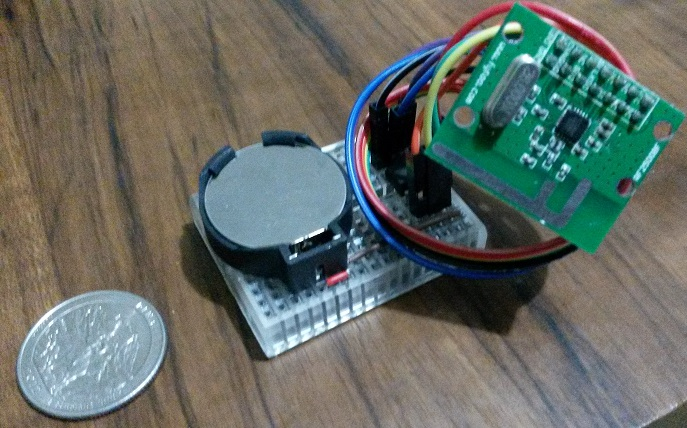
\includegraphics[width=0.5\textwidth]{images/phone_picture.png}
  \caption{Node on a breadboard.
  \label{img:flowchart}
  }
\end{figure}

While 20 nodes are fine for hardware simulation, we wanted to investigate a more realistic number of sensor nodes. However, it is not possible to install ContikiOS onto our MCU due to memory limitations. We attempted to enable intercommunication by acquiring an ATMega128RFA1. This microcontroller is directly supported by Contiki. Though it has a Zigbee-compatible transceiver on board, we would still need to provide it with a CC2500 transceiver as the Zigbee-compatible onboard transceiver is incompatible with ours. This plan ran into an early critical problem: the ATMega does not have on-board support for USB. This makes getting output from them extremely difficult. A solution could not be found in time, so this part remains unfinished.

\subsection{Throughput}

%
% bill of materials
%
\begin{table*}%[h!]
  \begin{center}
  
  \begin{tabular}{| c | c | c | c |}

  \hline
  \textbf{Number of Nodes} & \textbf{Success rate} & \textbf{Latency (s)} \\
  \hline

  20               & 26.5\% & 160 \\
  200              & 4.5\% & 114 \\

  \hline
  
  \end{tabular}  
  \end{center}
  \caption{Simulation results with randomly placed nodes.
  \label{table:bill}
  }
\end{table*}

The throughput was observed by simulating in Contiki to observe the throughput possible given a duty cycle.  The heart-beat
protocol produced consistent throughput during our energy simulations, although there were still instances of corrupted packets
propagating despite the use of checksums.  Our initial tests attempted to simulate these protocols with 200 randomly placed nodes using the
Cooja~\cite{cooja} network simulator using the standard radio broadcast model, for 30 minutes.  The nodes received simulated
temperature data every 8 minutes from their sensor and attempt to update the network about it, while keeping track other nodes'
data as well.  The heartbeat protocol was unable
to establish a global pattern.  The random sleep cycle model was able to connect and send data, but the majority of the data
did not reach the entire network.  Of the data that remained persistent on the network, it was only found on 22\% of the nodes,
on average.  For the successfully transferred data, the average throughput was observed to be 144 ms, however.  On a smaller
network with 10 randomly placed nodes the results improve a little, and could probably be improved further by manually placing
nodes and managing the network set-up.
